\begin{center}
    {\LARGE \textbf{2010有机化学}} \\[2ex]
    {\large 时量180分钟 \quad 满分150分}
\end{center}

\vspace{0.5cm}
\noindent\textbf{注意事项:}
\begin{enumerate}[label=\arabic*., parsep=0pt, itemsep=0pt]
    \item 答题前,考生先将自己的姓名、学号、考场号、座位号填写在答题卡上,将条形码准确粘贴在考生信息条形码粘贴区。
    \item 考试结束后,将本试卷与答题纸一并收回。
    \item 回答各个问题时,将答案写在答题纸上,写在本试卷上无效。
\end{enumerate}

\vspace{0.5cm}
\noindent\textbf{一、完成反应(30 pts.)}

\begin{enumerate}[label=\arabic*., itemsep=3ex]
    \item 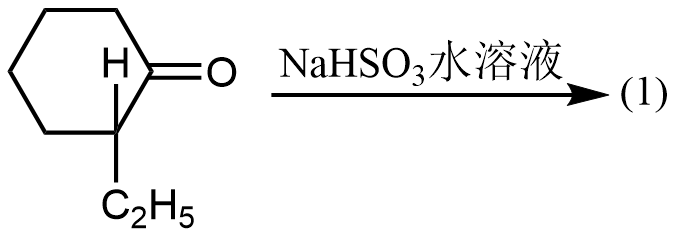
\includegraphics[scale=0.38, valign=c]{./Figure/2010/2010_1_1.png} 
    \item 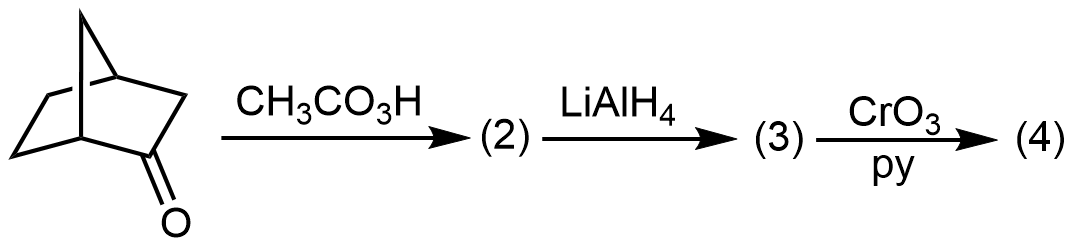
\includegraphics[scale=0.38, valign=c]{./Figure/2010/2010_1_2.png}
    \item 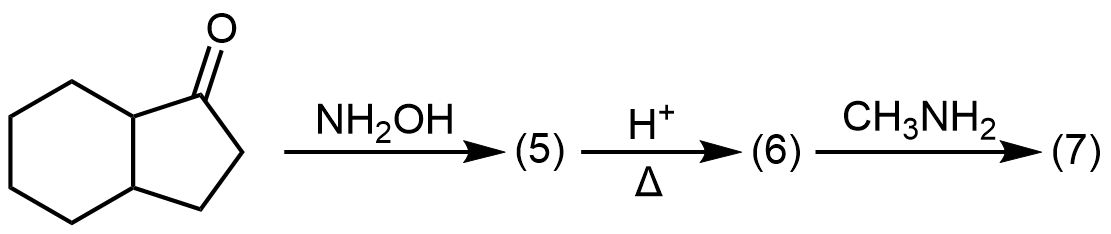
\includegraphics[scale=0.38, valign=c]{./Figure/2010/2010_1_3.png}
    \item 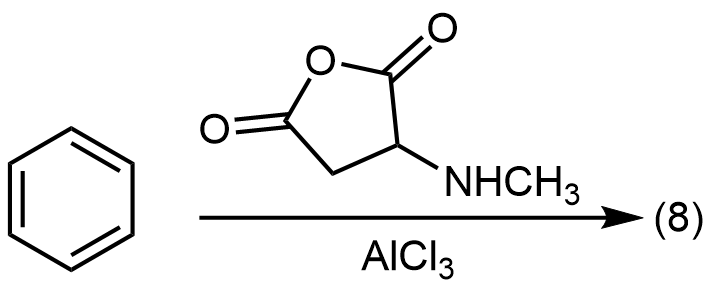
\includegraphics[scale=0.38, valign=c]{./Figure/2010/2010_1_4.png}
    \item 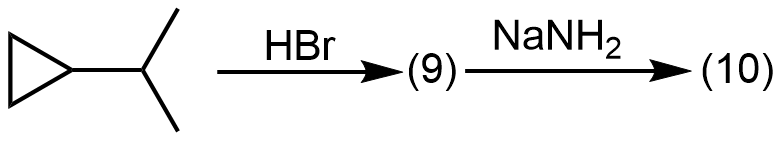
\includegraphics[scale=0.38, valign=c]{./Figure/2010/2010_1_5.png}
    \item 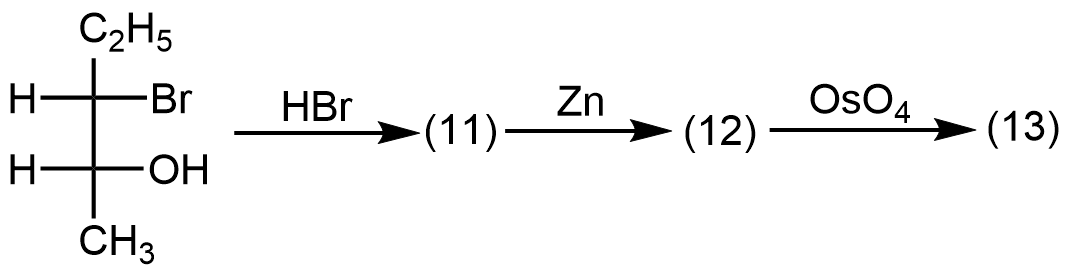
\includegraphics[scale=0.38, valign=c]{./Figure/2010/2010_1_6.png}
    \item 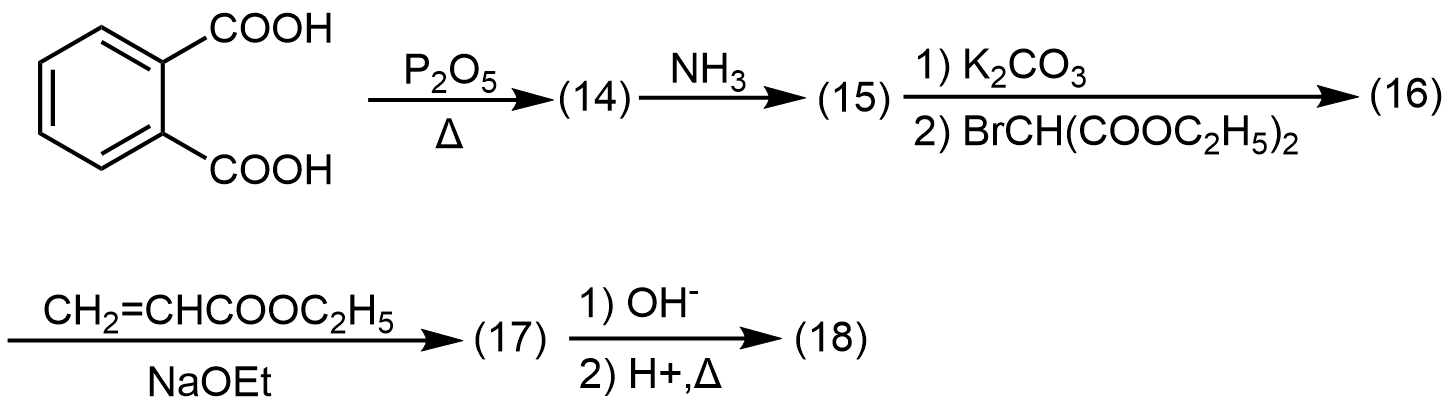
\includegraphics[scale=0.38, valign=c]{./Figure/2010/2010_1_7.png}
    \item 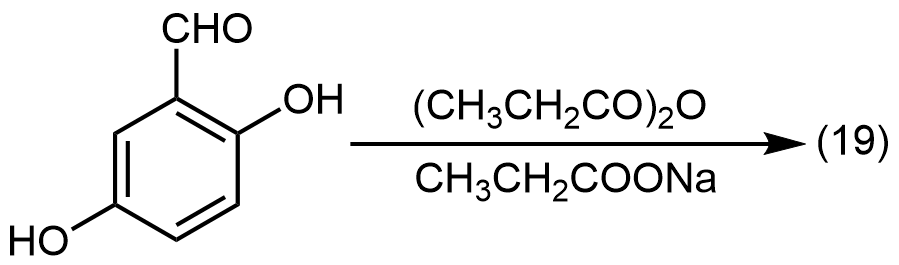
\includegraphics[scale=0.38, valign=c]{./Figure/2010/2010_1_8.png}
    \item 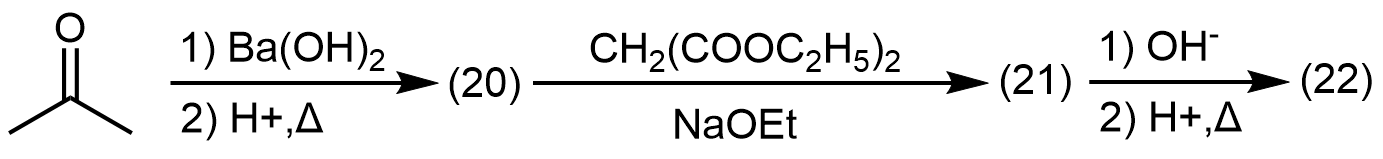
\includegraphics[scale=0.38, valign=c]{./Figure/2010/2010_1_9.png}
    \item 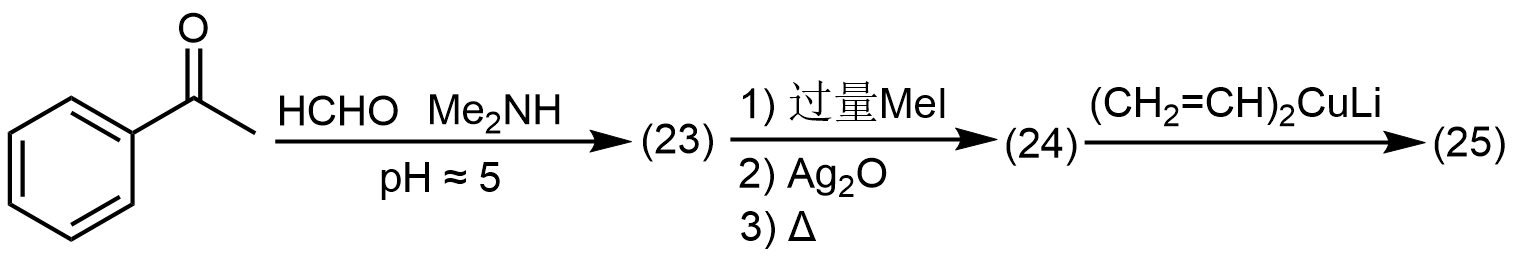
\includegraphics[scale=0.38, valign=c]{./Figure/2010/2010_1_10.png}
    \item 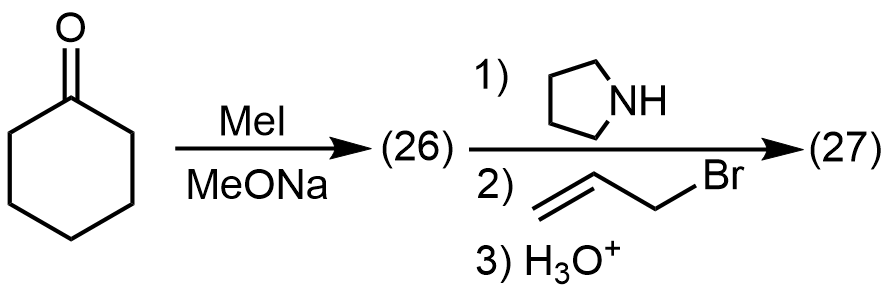
\includegraphics[scale=0.38, valign=c]{./Figure/2010/2010_1_11.png}
    \item 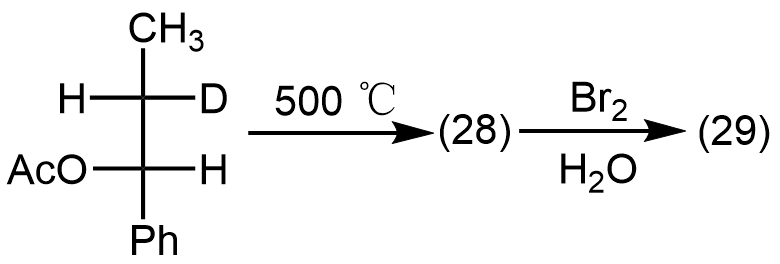
\includegraphics[scale=0.38, valign=c]{./Figure/2010/2010_1_12.png}
    \item 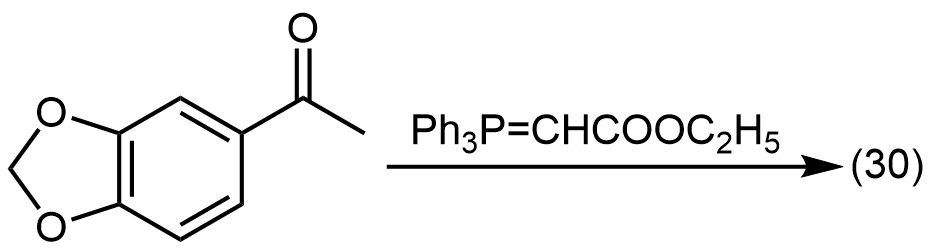
\includegraphics[scale=0.38, valign=c]{./Figure/2010/2010_1_13.png}
\end{enumerate}

\vspace{0.5cm}
\noindent\textbf{二、机理题(30 pts.)}

\begin{enumerate}[label=\arabic*., start=1, itemsep=1.5ex]
    \item 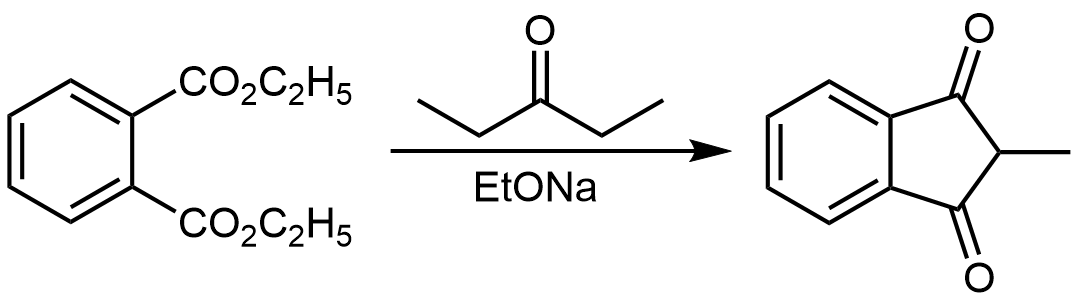
\includegraphics[scale=0.38, valign=c]{./Figure/2010/2010_2_1.png}
    \item 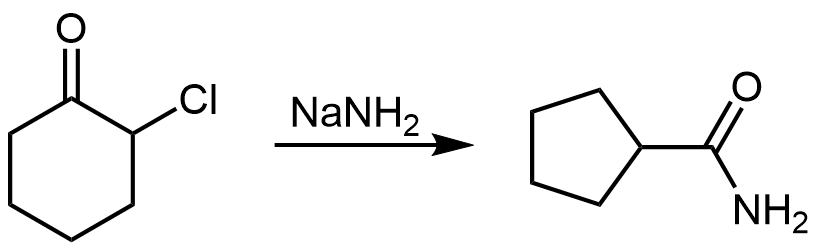
\includegraphics[scale=0.38, valign=c]{./Figure/2010/2010_2_2.png}
    \item 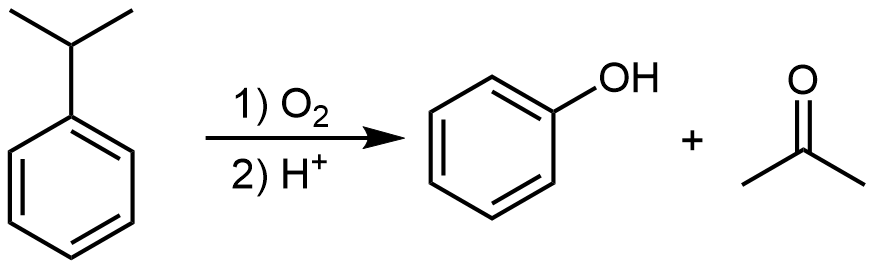
\includegraphics[scale=0.38, valign=c]{./Figure/2010/2010_2_3.png}
\end{enumerate}

\vspace{0.5cm}
\noindent\textbf{三、合成题(30 pts.)}

\begin{enumerate}[label=\arabic*., start=1, itemsep=1.5ex]

    \begin{figure}[htbp]
        \centering
        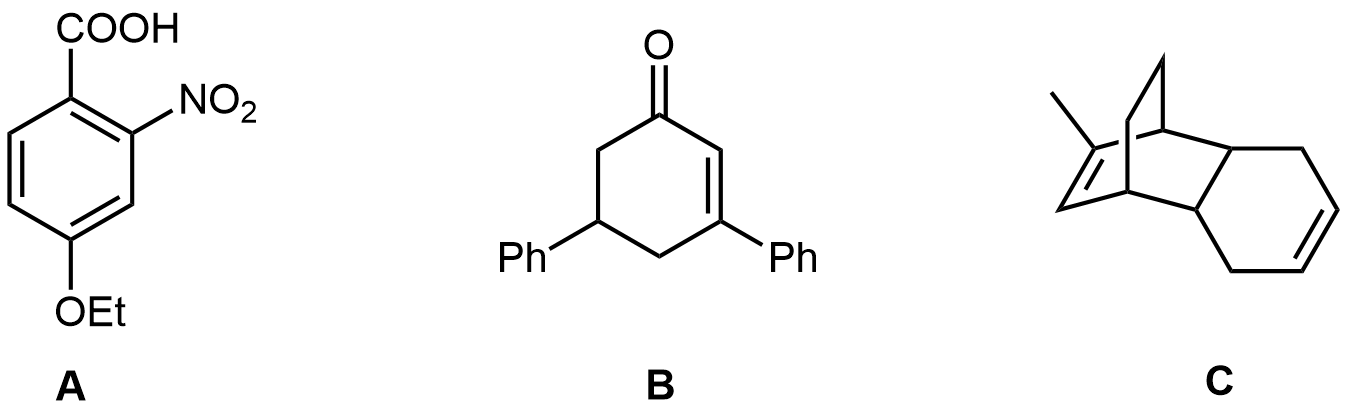
\includegraphics[scale=0.38]{./Figure/2010/2010_3.png}
    \end{figure}
    \item 以苯为主要原料合成\textbf{A}
    \item 以苯以及小于等于3个碳的有机原料合成\textbf{B}
    \item 以小于等于2个碳的有机原料合成\textbf{C}
\end{enumerate}

\vspace{0.5cm}
\noindent\textbf{四、综合题(40 pts.)}

\begin{enumerate}[label=\arabic*., start=1, itemsep=1.5ex]
    \item 简述呋喃的乙酰化反应发生在$\alpha$ 位的原因(6 pts.)
    \item 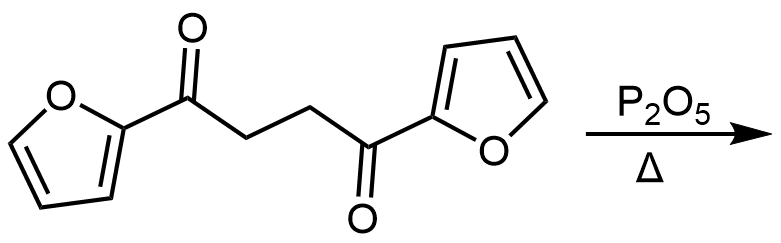
\includegraphics[scale=0.38, valign=c]{./Figure/2010/2010_4_2.png}(2 pts.)
    \item 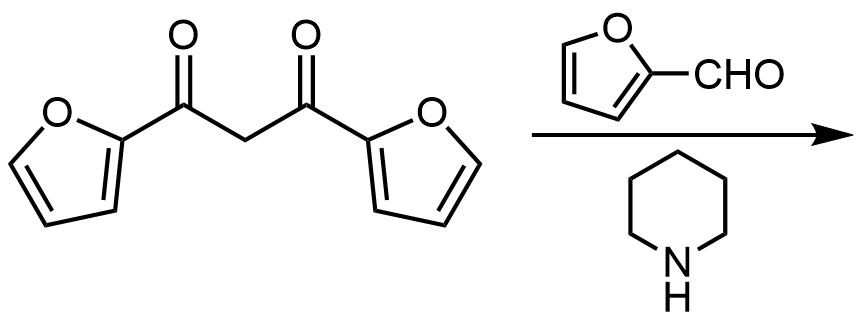
\includegraphics[scale=0.38, valign=c]{./Figure/2010/2010_4_3.png}(2 pts.)
    \item 以$\alpha$ -乙酰呋喃为原料，并可选用乙酸乙酯、乙醇、\ce{Br2}、\ce{I2}和其他必要的试剂等原料，合成化合物\textbf{A}和\textbf{B}。(12 pts.) 
    \begin{figure}[htbp]
        \centering
        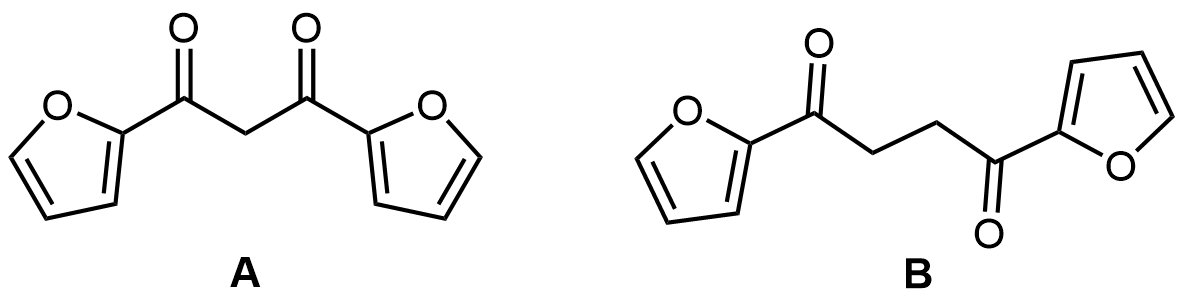
\includegraphics[scale=0.38]{./Figure/2010/2010_4_4.png}
    \end{figure}
    \item 写出反应1和反应2的机理(12 pts.)
    \begin{figure}[htbp]
        \centering
        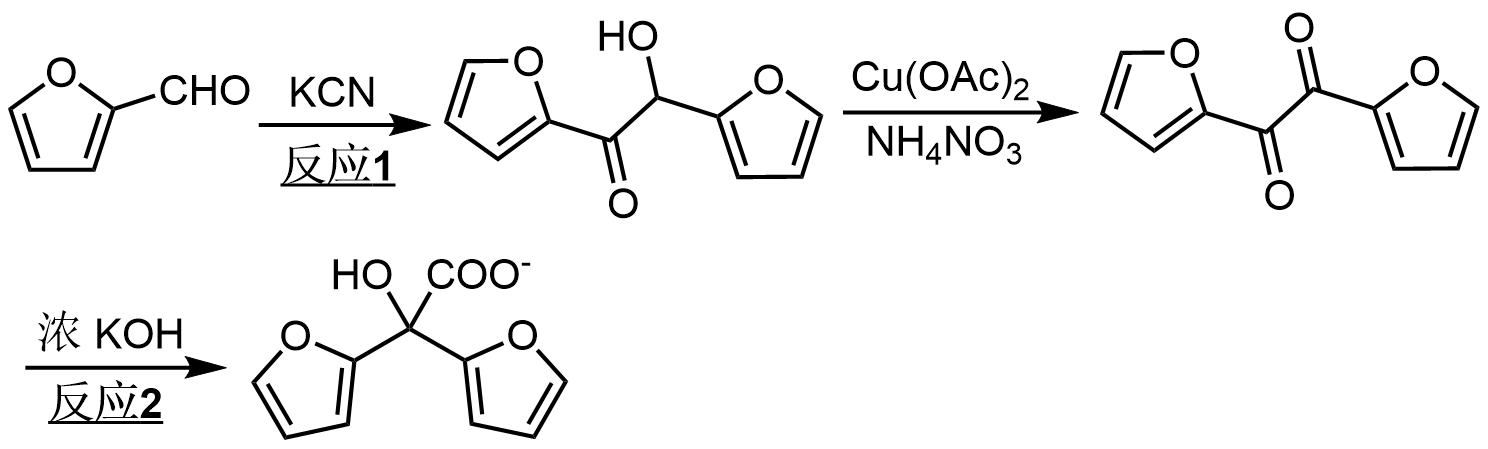
\includegraphics[scale=0.38]{./Figure/2010/2010_4_5.png}
    \end{figure}
    \item 设计合成路线完成下面的转化(6 pts.)
    \begin{figure}[htbp]
        \centering
        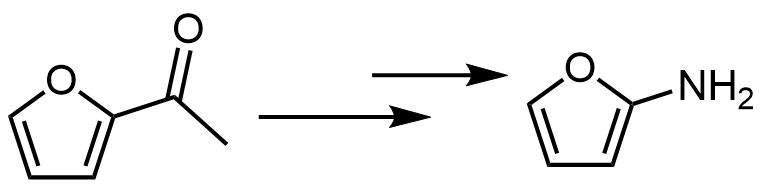
\includegraphics[scale=0.38]{./Figure/2010/2010_4_6.png}
    \end{figure}
\end{enumerate}

\vspace{0.5cm}
\noindent\textbf{五、实验题 略}